

\titlespacing*{\section}{0pt}{0.1cm}{0cm}
\graphicspath{{image/}}
\renewcommand{\headrulewidth}{0pt}
\renewcommand{\footrulewidth}{0pt}


\pagestyle{fancy}
\fancyhf{} % Очистить текущие настройки
\fancyfoot[L]{\thepage} % Номер страницы в левом нижнем углу
\fancyfoot[C]{} % Убрать центральный текст
\fancyfoot[R]{} %
\setlength{\footskip}{15pt}


\begin{center}
    \huge
    \textbf{Решения задач}
    \\
    
    \Large
    \textbf{M444,M445;Ф458-Ф461}
\end{center}
\section*{}

\begin{tabular}{p{50mm} p{120mm}}
        
    \textbf{M444} a) \textit{На рисунке 1 четыре прямые разбивают плоскость на одиннадцать областей: четырезугольник(1), 2 треугольника(2 и 3), три угла (4, 5 и 6), четыре <<бесконечных треугольника>> --- области, ограниченные каждая отрезком и двумя лучами (7, 8, 9, и 10) и <<бесконечный четырехугольник>>--- область, ограниченную двумя отрезками и двумя лучами(11).}
    
    \textit{Будет ли сказанное верно для любых четырех прямых на плоскости, среди которых нет параллельных и нет прямых, проходящих через одну точку?}
    
    \textit{б) Три больших круга, не проходящие через одну точку разбивают сферу на восемь треугольников. На какие области разбивают сферу четыре больших круга, никакие три из которых не проходят через одну точку? (Большим кругом на сфере называют окружность, являющуюся пересечением сферы с плоскостью, проходящей через центр сферы, рис.2.)}
    
    \textit{в) На какие области могут разбить сферу пять больших кругов никакие три из которых не проходят через одну точку?}

    
    \section*{}
    \vspace{-4mm}
    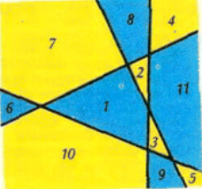
\includegraphics[width=1.0\linewidth]{img}
    Рис. 1.
& 
    Будем говорить, что несколько прямых на плоскости (или больших кругов на сфере) находятся в общем положении, если все они попарно пересекаются, причем в различных точках. Выпуклую фигуру на плоскосоти, ограниченную двумя лучами и n--1 отрезками, будем для краткости называть n-углом (у n-угла n вершин, 1-угол --- это угол в обычном смысле). Перейдем к решению задач.

    а) Нетрудно убедиться в том, что для любых четырех прямых общего положения разбиение будет всегда одинаковым:
    \section*{}
    \vspace{-4mm}
    \renewcommand{\arraystretch}{2}
\begin{center}
\begin{tabularx}{\linewidth}{|>{\centering\arraybackslash}p{2.125cm}|>{\centering\arraybackslash}p{2.125cm}|>{\centering\arraybackslash}X|>{\centering\arraybackslash}X|>{\centering\arraybackslash}X|}
    \hline
    4-угольников & 3-угольников & Углов & 2-углов & 3-углов \\ \hline
    1 & 2 & 3 & 4 & 1 \\ \hline
\end{tabularx}
\end{center}



\section*{}
--- таким же, как на рисунке 1. После нескольких минут, проведенных за рисованием четверок прямых, это становится совершенно очевидным. Рассуждения, присланные по этому поводу читателями, очень разнообразны, но они показывают, что записать короткое и в то же время убедительное доказательство этого очевидного факта не так просто. В самом деле, если не ссылаться на чертеж пришлось бы при формальном доказательстве опираться прямо на геометрические аксиомы, характеризующие расположение отрезков и прямых на плоскости --- решение получилось бы довольно длинным. Мы не будем столь педантичны, а проведем лишь набросок доказательства, по-видимому, вполне убедительного. По существу, именно так обычно и поступают в решениях геометрических задач, <<близких к аксиомам>>.

Докажем, что одной из частей, на которые четыре прямые общего положения делят плоскость, будет четырехугольник. Этого достаточно для решения задачи: ясно, что при продолжении сторон любого выпуклого четырехугольника без параллельных сторон мы получим такие же 10 остальных областей, как на рисунке 1.

Проведем сначала три прямые общего положения. Они попро пересекаются в трех точках A, B и C. Четвертая прямая l делит плоскость на две полуплоскости. Если две из трех точек A, B, C лежат в одной полуплоскости, а одна (скажем, A) --- в другой то прямая l отсекает от треугольника ABC четырехугольник (BCED; рис. 3, \textit{a}). Если  все три точки лежат в одной полуплоскости, причем A --- дальше от l, чем B и С, то прямая l отсекает от 2-угла с вершинами B и С четырехугольник (BCED; рис. 3, \textit{б}).

\hspace{0.5cm}Для каждой из задач б) и в) мы приведем по два решения, причем вторые решения будут использовать задачу а), а первые --- нет.

б) О т в е т: \textit{разбиение всегда одинаковое; оно состоит из 14 областей --- 6 четырехугольников и 8 треугольников.}

П е р в о е\hspace{0.3cm}р е ш е н и е: Проведем сначала три больших круга 1, 2, 3 (см. рис. 2). Они делят сферу на восемь треугольников. Выясним, сколько из них будет пересекать четвертый большой круг 4, находящийся в общем положении с 1, 2 и 3. Для этого достаточно узнать, на сколько отдельных кусков будет разбит круг 4 точками пересечения с тремя другими. Каждые два больших круга пересекаются пересекаются в двух диаметрально противоположных точках. Поэтому большой круг 4 пересекает три других больших круга 1, 2, 3 всего в шести точках, т.е. разбиваются ими всего на шесть дуг. Таким образом,
\end{tabular}
\fancyfoot[L]{32}

\newpage
\thispagestyle{empty}
\begin{tabular}{p{50mm} p{120mm}}

\textit{ке 7. Пусть M --- многоугольник с вершинами в центрах окружностей. Окрасим в красный цвет те окружности или их части (дуги), которые лежат внутри М. Покажите, что сумма градусных величин красных дуг равна $C\cdot180^{\circ}$, где $C=C(M)$---целое число, и дайте этому числу геометрическую интерпретацию.}
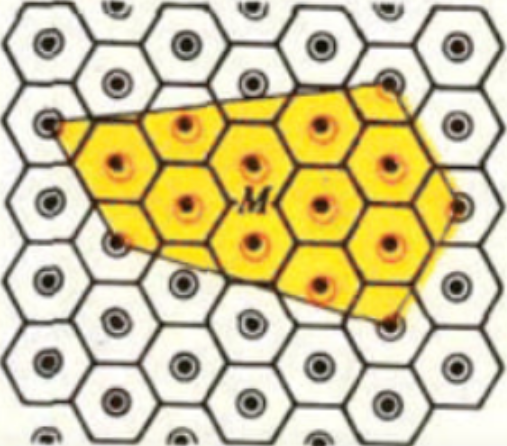
\includegraphics[width=1.0\linewidth]{image2}
Рис. 7

&

многоугольников $A_1$, ...,$A_k$ (с вершинами в узлах):
{
\vspace{-4mm}
$M=\bigcup\limits_{i=l}^k A_i$, то $$C(M)=C(A_1)+...+C(A_k);$$
}

{
\vspace{-3mm}
про такую функцию говорят, что она \textit{аддитивна}. Отсюда следует, что если многоугольник М с вершинами в узлах представлен в виде объединения многоугольников $B_1$, ...,$B_l$ ($A_i$ и $B_j$ --- с вершинами в узлах) --- см. рисунок 8; т.е. если 
}

{
\vspace{-2mm}
\begin{equation*}
    M = \bigcup\limits_{i=1}^k A_i \setminus \bigcup\limits_{j=1}^k B_j\text{ причем }\bigcup B_j \subset \bigcup A_i
    \tag{*}
\end{equation*}
}

{
\vspace{-2mm}
(здесь $\setminus$ --- значок \textit{разности множеств} или \textit{дополнения}), то 
}
\vspace{-3mm}
$$C(M)=\sum\limits_{i=1}^kC(A_i) - \sum\limits_{j=1}^kC(B_j)\text{.}$$

{
\vspace{-3mm}
Ниже мы покажем, что всякий многоугольник М (с вершинами в узлах) представляется в виде (*) где $A_i$ и $B_j$ --- треугольники. Поэтому утверждение задачи достаточно доказать для треугольников T с вершинами в узлах.

Итак, покажем что C(T) --- целое число. Впишем треугольник T в параллелограмм П со сторонами, параллельными сторонам решетки. Поскольку вершины T находятся в узлах, вершины П находятся в узлах. 
Представим параллелограмм П в виде объединения треугольника T и треугольников $T_{\text{П}}$, у которых две стороны параллельны сторонам решетки
}
\end{tabular}

